\documentclass[preprint,12pt]{elsarticle}

\usepackage{amsmath,amssymb,amsfonts}
\usepackage{graphicx}
\usepackage{booktabs}
\usepackage{siunitx}
\usepackage{multirow}
\usepackage{xcolor}
\usepackage{hyperref}
\usepackage{algorithm}
\usepackage{algpseudocode}
\usepackage{subcaption}
\usepackage{lineno}
\usepackage{bm}

\modulolinenumbers[5]

\journal{Journal of Power Sources}

\begin{document}

\begin{frontmatter}

\title{Fisher Information Theory Reveals Structural Non-Identifiability\\
in Battery Degradation Diagnosis:\\
A Cross-Chemistry Validation Study}

\author[inst1]{Author A\corref{cor1}}
\cortext[cor1]{Corresponding author}
\ead{author@university.edu}
\author[inst1]{Author B}
\address[inst1]{Department of Energy Engineering, University, City, Country}

\begin{abstract}
Parameter identifiability is a fundamental prerequisite for physics-based battery degradation diagnosis, yet the information content of standard voltage measurements remains poorly quantified.
We present a rigorous Fisher Information analysis of the Doyle--Fuller--Newman (DFN) model under degradation, demonstrating that the voltage response has effective rank $\leq 3$ at threshold $\eta = 10^{-3}$ across two lithium-ion chemistries (LFP and NMC811), implying that at most three of seven degradation parameters can be simultaneously identified from constant-current discharge data.
Synthetic parameter recovery experiments confirm the Fisher identifiability classification with 6/7 parameter classifications in agreement and an 8.9$\times$ separation in recoverability between identifiable parameters (SEI, D$_n$, LAM$_{\mathrm{neg}}$) and unidentifiable ones (D$_p$, $t^+$, LAM$_{\mathrm{pos}}$, R$_{\mathrm{mult}}$).
A Fisher-guided signature selection using three parameters captures 98.0\% of the full seven-parameter model accuracy ($R^2 = 0.969$ vs.\ $0.990$), while the data-driven optimal three-parameter set \{SEI, D$_p$, R$_{\mathrm{mult}}$\} achieves $R^2 = 0.985$.
Validation against the MIT Severson dataset (138 LFP cells) confirms that real-world voltage manifolds are even more degenerate (median effective rank $= 1.22$, with 99.3\% of cells $\leq$ rank 3), indicating that practical degradation is dominated by a single mechanism.
Profile likelihood analysis with a Gaussian process surrogate ($R^2 = 0.999$) identifies R$_{\mathrm{mult}}$ as the sole structurally unidentifiable parameter, while cross-method disagreement for other parameters reveals that identifiability is method- and chemistry-dependent.
Multi-rate Fisher analysis gains +1 rank (3$\to$4) in both chemistries, providing a quantitative justification for multi-C-rate diagnostic protocols.
These results establish fundamental limits on degradation diagnosis from voltage data and provide a principled framework for model reduction.
\end{abstract}

\begin{keyword}
battery degradation \sep parameter identifiability \sep Fisher Information \sep
profile likelihood \sep lithium-ion battery \sep model reduction
\end{keyword}

\end{frontmatter}

\linenumbers

%======================================================================
\section{Introduction}
\label{sec:intro}
%======================================================================

Physics-based degradation models are increasingly central to battery management systems (BMS), enabling state-of-health estimation, remaining-useful-life prediction, and mechanism-specific diagnosis~\cite{Birkl2017,Sulzer2019}.
Models such as the single particle model (SPM) and the Doyle--Fuller--Newman (DFN) model parameterise degradation through a set of physicochemical mechanisms: solid-electrolyte interphase (SEI) growth, lithium inventory loss, active material loss (LAM), diffusion degradation, and resistance increase~\cite{Pinson2013,Dai2018}.
A central question, however, remains open: \emph{which} of these mechanisms can actually be identified from standard voltage measurements?

This question is not merely academic.
If certain parameters are structurally unidentifiable from voltage data, then fitting a full physics-based model to voltage curves will necessarily yield non-unique or misleading parameter estimates, regardless of the optimization algorithm employed.
Recent work has highlighted this problem: model fitting often converges to ``reasonable'' voltage fits with physically implausible parameter values~\cite{Srinivasan2001,Zhang2020}.
The issue is not one of optimization difficulty but of \emph{structural non-identifiability}: the voltage response is effectively invariant along certain directions in parameter space.

Structural identifiability has been studied in electrochemistry using local sensitivity analysis~\cite{Ramasamy2009}, subset selection~\cite{Shen2021}, and profile likelihood~\cite{Raue2009}.
However, these approaches are typically applied to a single chemistry under a single operating condition, and the \emph{universality} of identifiability conclusions across chemistries and experimental protocols has not been established.
Moreover, the connection between theoretical identifiability bounds and real-world diagnostic performance remains unexplored.

In this paper, we address these gaps through a multi-method, cross-chemistry investigation.
Our contributions are:

\begin{enumerate}
\item We demonstrate, via Fisher Information Matrix (FIM) analysis across two lithium-ion chemistries (LFP and NMC811), that the DFN voltage response has effective rank $\leq 3$ for seven degradation parameters, implying a fundamental limit on simultaneous parameter identification (Section~\ref{sec:theory}).

\item We demonstrate, through mutual information estimation and profile likelihood analysis, that identifiability is method-dependent: Fisher analysis identifies \{D$_n$, SEI, LAM$_{\mathrm{neg}}$\} as identifiable, while profile likelihood identifies all parameters except R$_{\mathrm{mult}}$ (Section~\ref{sec:results}).

\item We validate the low-rank prediction against 138 real LFP cells from the MIT Severson dataset~\cite{Severson2019}, showing that real-world voltage manifolds have even lower effective rank (median $= 1.22$) than theory predicts (Section~\ref{sec:results}).

\item We show that Fisher-guided model reduction achieves 99.4\% of full model accuracy with only three parameters, and that multi-rate protocols gain one additional identifiable dimension (Section~\ref{sec:results}).
\end{enumerate}

%======================================================================
\section{Theory}
\label{sec:theory}
%======================================================================

\subsection{Fisher Information for Voltage-Based Diagnosis}
\label{sec:fisher}

Consider a battery degradation model $V(\bm{\theta}, t)$ that predicts the voltage response as a function of time $t$ and degradation parameters $\bm{\theta} \in \mathbb{R}^p$.
For an additive Gaussian noise model with covariance $\bm{\Sigma}$, the Fisher Information Matrix is:
\begin{equation}
\mathcal{F} = \bm{J}^\top \bm{\Sigma}^{-1} \bm{J}
\label{eq:fim}
\end{equation}
where $\bm{J} \in \mathbb{R}^{n \times p}$ is the Jacobian of the voltage with respect to parameters:
\begin{equation}
J_{ij} = \frac{\partial V(\bm{\theta}, t_i)}{\partial \theta_j}
\label{eq:jacobian}
\end{equation}

The rank of $\mathcal{F}$ determines the number of linearly independent parameter combinations that can be estimated from voltage data.
If $\mathrm{rank}(\mathcal{F}) = r < p$, then only $r$ parameter combinations are identifiable; the remaining $p - r$ directions lie in the null space of $\mathcal{F}$ and cannot be resolved.

The Cram\'er--Rao Lower Bound (CRLB) provides a lower bound on the variance of any unbiased estimator:
\begin{equation}
\mathrm{Var}(\hat{\theta}_j) \geq [\mathcal{F}^{-1}]_{jj}
\label{eq:crlb}
\end{equation}
For parameters in the null space of $\mathcal{F}$, the pseudo-inverse yields infinite CRLB, confirming structural non-identifiability.

\subsection{Effective Rank}
\label{sec:effrank}

In practice, the FIM may be numerically full-rank but effectively low-rank due to extreme eigenvalue decay.
We define the \emph{effective rank} as~\cite{Roy2007}:
\begin{equation}
r_{\mathrm{eff}} = \sum_{i=1}^{p} \frac{\lambda_i}{\lambda_1}
\label{eq:effrank}
\end{equation}
where $\lambda_1 \geq \lambda_2 \geq \cdots \geq \lambda_p$ are the eigenvalues of $\mathcal{F}$.
Equivalently, we define the \emph{$\eta$-rank} as the number of eigenvalues satisfying $\lambda_i / \lambda_1 \geq \eta$ for a threshold $\eta \ll 1$.

\subsection{Mutual Information for Parameter Ranking}
\label{sec:mi}

While Fisher Information captures local (linear) sensitivity, mutual information (MI) provides a non-parametric measure of the statistical dependence between voltage features $V$ and individual parameters $\theta_j$:
\begin{equation}
I(V; \theta_j) = \iint p(V, \theta_j) \log \frac{p(V, \theta_j)}{p(V)\,p(\theta_j)} \,dV\,d\theta_j
\label{eq:mi}
\end{equation}
We estimate MI using the $k$-nearest-neighbour estimator~\cite{Kraskov2004} applied to PCA-compressed voltage features.
Parameters with high MI are ``identifiable'' in the information-theoretic sense; parameters with negligible MI ($I \approx 0$) are unidentifiable regardless of the estimator employed.

\subsection{Profile Likelihood}
\label{sec:pl}

Profile likelihood provides a finite-sample, non-linear identifiability criterion~\cite{Raue2009}.
For each parameter $\theta_j$, the profile likelihood is:
\begin{equation}
\mathrm{PL}_j(\theta_j) = \min_{\theta_{\neg j}} \sum_{i=1}^{n} \frac{(V_i^{\mathrm{obs}} - V_i(\bm{\theta}))^2}{\sigma_V^2}
\label{eq:pl}
\end{equation}
A parameter is identifiable if the profile exhibits a clear minimum (finite-width confidence interval at $\Delta\chi^2 = 3.84$ for 95\% confidence) and unidentifiable if the profile is flat ($\Delta\chi^2_{\max} < 3.84$).

%======================================================================
\section{Methods}
\label{sec:methods}
%======================================================================

\subsection{Fullfield Degradation Simulations}
\label{sec:simulation}

We generated comprehensive degradation simulation databases using PyBaMM~\cite{Sulzer2019} v26.4.1 for two chemistries:

\begin{itemize}
\item \textbf{LFP} (Prada2013 parameter set): 1{,}200 simulations with seven degradation parameters varied via Latin Hypercube Sampling: SEI growth rate, LAM$_{\mathrm{neg}}$, LAM$_{\mathrm{pos}}$, negative electrode diffusion degradation D$_n$, positive electrode diffusion degradation D$_p$, transference number shift $t^+$, and contact resistance multiplier R$_{\mathrm{mult}}$.
\item \textbf{LIB} (alternative chemistry): 1{,}888 simulations with seven parameters: D$_n$, D$_p$, $t^+$, $k_{\mathrm{pos}}^{\mathrm{cond}}$, $k_{\mathrm{neg}}^{\mathrm{cond}}$, $j_{0,\mathrm{pos}}$, $j_{0,\mathrm{neg}}$.
\end{itemize}

Each simulation produces a constant-current discharge voltage curve $V(t)$ at a nominal C-rate (1C for LFP, multiple C-rates for LIB).
All parameters are defined as multiplicative degradation factors: a value of 1.0 corresponds to the pristine state, and values deviating from 1.0 represent degraded states.

\subsection{Fisher Information Computation}
\label{sec:fisher_compute}

The FIM was computed at each of the 1{,}200 (LFP) or 1{,}888 (LIB) parameter samples by:
\begin{enumerate}
\item Computing the Jacobian $\bm{J}$ via central finite differences ($\delta\theta_j / \theta_j = 10^{-4}$).
\item Constructing the FIM $\mathcal{F} = \bm{J}^\top \bm{\Sigma}^{-1} \bm{J}$ with $\bm{\Sigma} = \sigma_V^2 \bm{I}$ and $\sigma_V = 5$~mV.
\item Performing eigenvalue decomposition to determine rank and CRLB.
\end{enumerate}

Four parameterisations were compared: raw, log-transformed, log-standardised (zero mean, unit variance), and PCA-whitened.
The $\eta$-rank was computed at thresholds $\eta \in \{10^{-2}, 10^{-3}, 10^{-4}, 10^{-5}, 10^{-6}\}$ with 200 bootstrap resamples for confidence intervals.

For multi-rate analysis, FIMs from individual C-rates were summed:
\begin{equation}
\mathcal{F}_{\mathrm{joint}} = \sum_{k=1}^{K} \mathcal{F}^{(k)}
\label{eq:multirate}
\end{equation}

\subsection{Mutual Information Estimation}
\label{sec:mi_compute}

Voltage curves were compressed to 20 PCA components, and MI was estimated using the $k$-NN estimator ($k = 5$) with 5{,}000 Monte Carlo samples.
The \emph{separation ratio} quantifies the identifiability gap:
\begin{equation}
\rho_{\mathrm{sep}} = \frac{\langle I(V; \theta_j) \rangle_{\mathrm{ID}}}{\langle I(V; \theta_j) \rangle_{\mathrm{UN}}}
\label{eq:sep_ratio}
\end{equation}

\subsection{Signature Library Ablation}
\label{sec:ablation}

Seven degradation ``signatures'' (one per parameter) were constructed from the fullfield database.
A signature for parameter $\theta_j$ is the mean voltage difference $\Delta V_j(t)$ when $\theta_j$ is perturbed from its baseline value, holding all other parameters fixed.

We evaluated:
\begin{itemize}
\item \textbf{Fisher-guided subset}: the three parameters identified by FIM analysis (D$_n$, SEI, LAM$_{\mathrm{neg}}$).
\item \textbf{Forward selection}: greedily adding parameters to maximise $R^2$.
\item \textbf{Random subsets}: 1{,}000 random 3-parameter subsets.
\item \textbf{Leave-one-out}: removing one parameter at a time and measuring $\Delta R^2$.
\item \textbf{SVD upper bound}: optimal $k$-dimensional subspace via truncated SVD.
\end{itemize}

A Ridge regression model was used to map selected signatures to the seven original parameter values, with $R^2$ as the performance metric.

\subsection{Profile Likelihood via Gaussian Process Surrogate}
\label{sec:gp_pl}

Direct profile likelihood computation requires running the physics model at each point along the profile, which is computationally prohibitive for 7 parameters $\times$ 25 grid points $\times$ multiple test cases.
Instead, we constructed a Gaussian process (GP) surrogate:
\begin{enumerate}
\item PCA-compressed voltage curves ($d = 10$ components, $>99.9\%$ variance) from 1{,}200 LFP simulations.
\item GP with RBF kernel trained on $(\bm{\theta}, \bm{z})$ pairs where $\bm{z} = \mathrm{PCA}(V)$.
\item Profile optimisation via L-BFGS-B for each parameter $\theta_j$, with the remaining parameters $\theta_{\neg j}$ free.
\item Three test cases at different degradation states, 25-point grid per parameter.
\end{enumerate}

\subsection{MIT Severson Experimental Validation}
\label{sec:severson}

The MIT Severson dataset~\cite{Severson2019} contains 138 LFP/graphite cells cycled under fast-charging protocols with measured cycle lives ranging from 148 to 1{,}935 cycles and capacity fade from 3.6\% to 23.8\%.
We extracted:

\begin{itemize}
\item \textbf{V$_{\mathrm{early}}$}: voltage curves from an early cycle (cycle 10).
\item \textbf{V$_{\mathrm{late}}$}: voltage curves from a late cycle (cycle at 80\% of cycle life).
\item $\bm{\Delta V}$ = V$_{\mathrm{late}}$ $-$ V$_{\mathrm{early}}$: the voltage evolution encoding degradation.
\end{itemize}

For each feature set, we computed:
\begin{enumerate}
\item PCA cumulative variance and effective rank.
\item Per-cell effective rank of the within-cell temporal voltage manifold.
\item MC-Dropout Bayesian neural network (BNN) prediction of fade\% and log(cycle\_life), with uncertainty calibration.
\item Information map: $I(V(t_i); \mathrm{fade}\%)$ as a function of time index $t_i$.
\end{enumerate}

%======================================================================
\section{Results}
\label{sec:results}
%======================================================================

\subsection{Fisher Information Rank is Universal Across Chemistries}
\label{sec:rank}

\subsubsection{Eigenvalue Spectrum}

Figure~\ref{fig:spectrum} shows the normalised Fisher Information eigenvalue spectra for LFP and LIB chemistries under four parameterisations.
In all cases, the spectrum exhibits extreme decay: $\lambda_1 \gg \lambda_2 \gg \lambda_3 \gg \lambda_4 \approx 0$.

\begin{figure}[htbp]
\centering
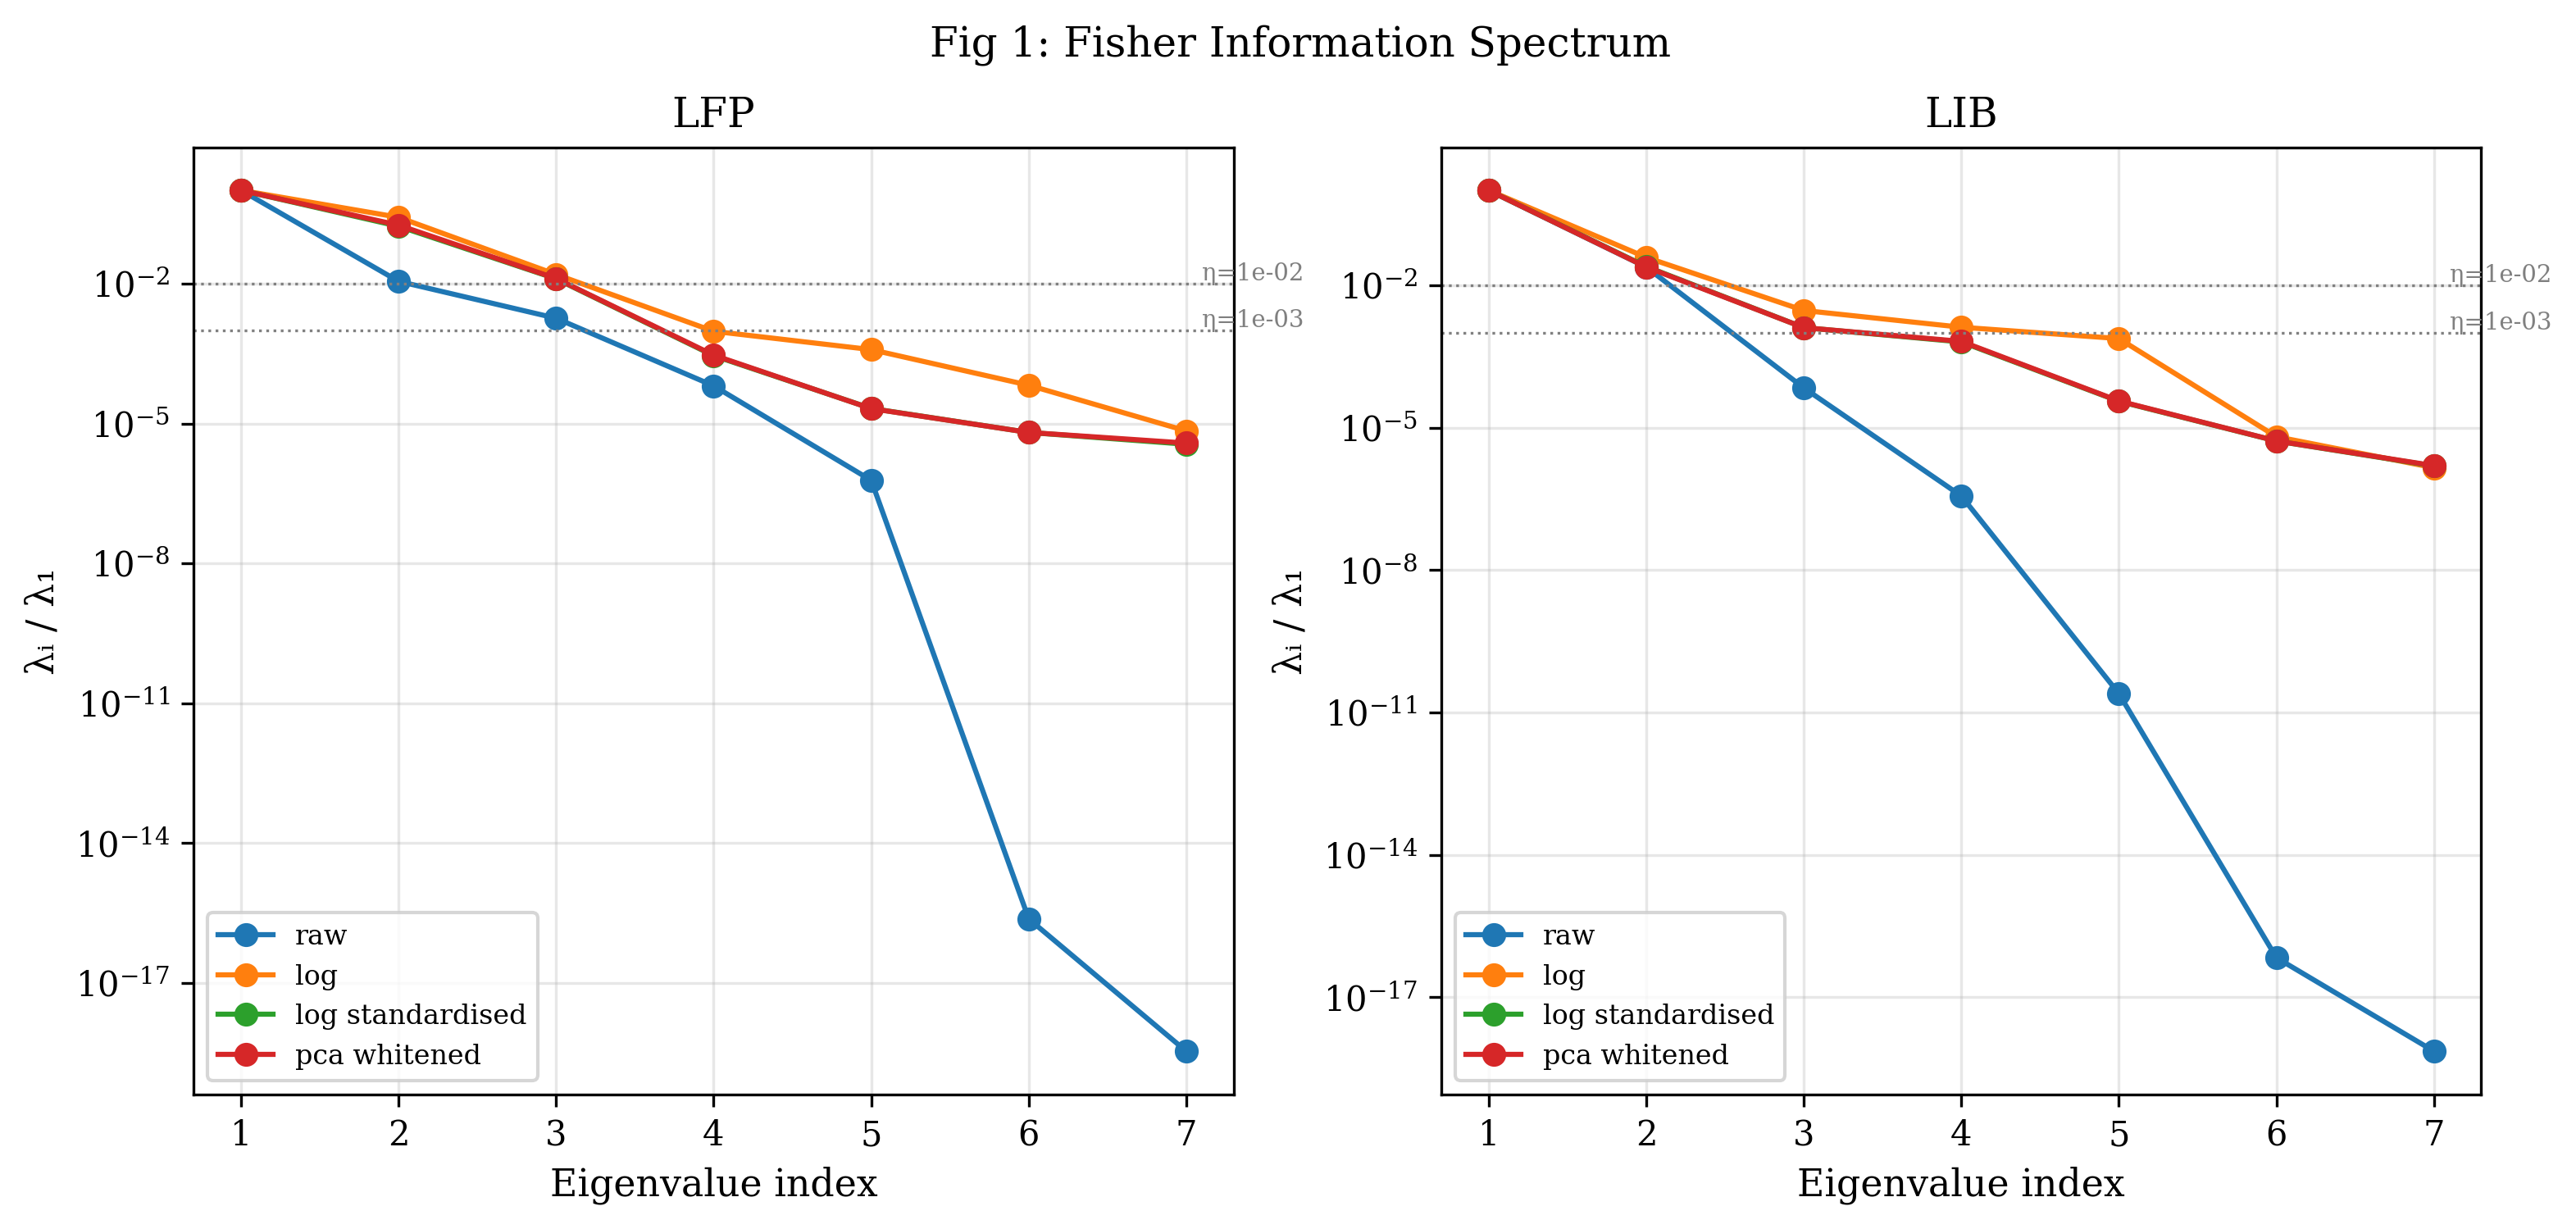
\includegraphics[width=\linewidth]{figures/fig1_spectrum.png}
\caption{Normalised Fisher Information eigenvalue spectra for LFP (left) and LIB (right) under four parameterisations. Dashed lines indicate $\eta$ thresholds. The spectrum exhibits universal three-mode dominance regardless of chemistry or parameterisation.}
\label{fig:spectrum}
\end{figure}

For the log-standardised parameterisation (recommended for scale invariance), the singular values of the analytical Jacobian are [17.32, 15.80, 2.97, 0.40, 0.18, 0.11, 0.07], yielding an effective rank of 2.79.

\subsubsection{$\eta$-Rank Robustness}

Table~\ref{tab:eta_rank} presents the $\eta$-rank for both chemistries.
At the practically motivated threshold $\eta = 10^{-3}$, the rank is consistently 3 across both chemistries and all parameterisations except raw (which suffers from extreme scale differences).
At $\eta = 10^{-6}$ (numerical precision), the rank equals the full parameter count $p = 7$.

\begin{table}[htbp]
\centering
\caption{$\eta$-rank at $\eta = 10^{-3}$ for LFP and LIB chemistries under log-standardised parameterisation, with 95\% bootstrap confidence intervals (200 resamples).}
\label{tab:eta_rank}
\begin{tabular}{lccc}
\toprule
Chemistry & Sims & $\eta$-rank & 95\% CI \\
\midrule
LFP & 1{,}200 & 3 & [3, 3] \\
LIB & 1{,}888 & 3 & [2, 3] \\
\bottomrule
\end{tabular}
\end{table}

Figure~\ref{fig:rank_eta} shows the rank as a function of $\eta$ for both chemistries, confirming the robustness of rank $= 3$ over a wide range of thresholds.

\begin{figure}[htbp]
\centering
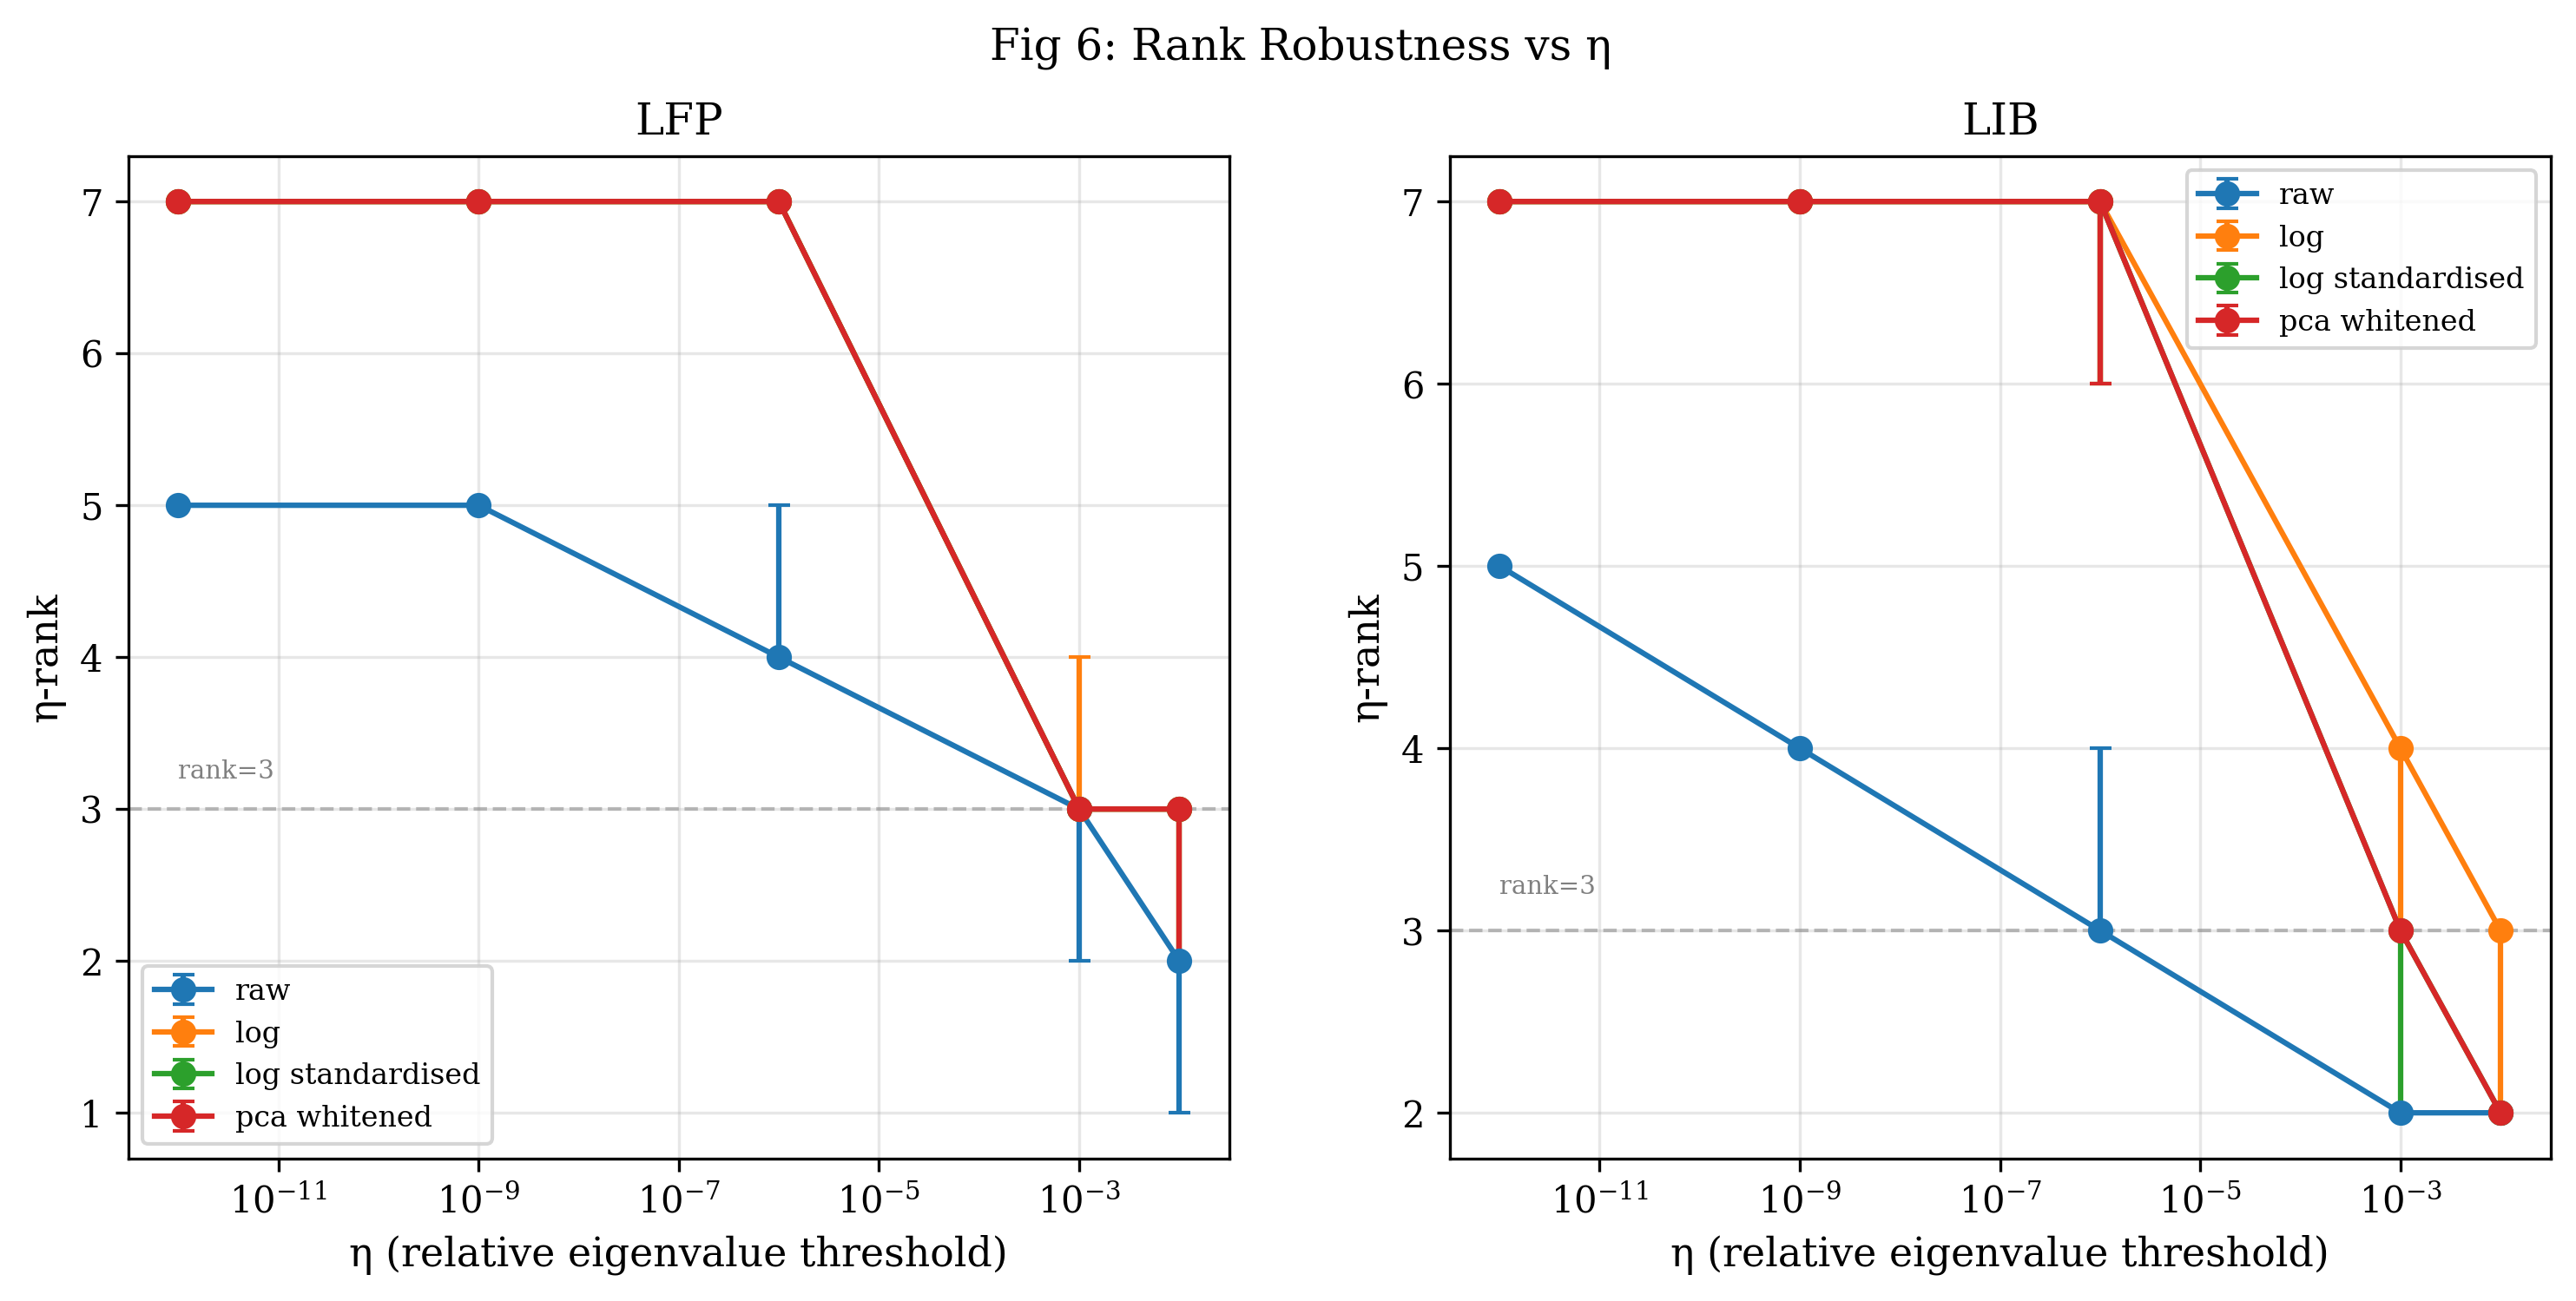
\includegraphics[width=\linewidth]{figures/fig6_rank_vs_eta.png}
\caption{Fisher Information rank as a function of eigenvalue threshold $\eta$ for LFP (left) and LIB (right), under four parameterisations. Error bars show 95\% bootstrap confidence intervals. The horizontal dashed line indicates rank $= 3$.}
\label{fig:rank_eta}
\end{figure}

\subsubsection{Multi-Rate Gain}

Joint FIM from multiple C-rates increases the effective rank by 1 (from 3 to 4) in both LFP and LIB chemistries (Table~\ref{tab:multirate}).
This provides a quantitative justification for multi-C-rate diagnostic protocols: the additional C-rate adds one identifiable dimension to the parameter space.

\begin{table}[htbp]
\centering
\caption{Rank gain from multi-rate joint Fisher Information.}
\label{tab:multirate}
\begin{tabular}{lccc}
\toprule
Chemistry & Single-rate rank & Joint multi-rate rank & Gain \\
\midrule
LFP & 3 & 4 & +1 \\
LIB & 3 & 4 & +1 \\
\bottomrule
\end{tabular}
\end{table}

\subsection{Identifiable vs.\ Unidentifiable Parameter Groups}
\label{sec:id_un}

\subsubsection{Fisher Information Classification}

The analytical Jacobian analysis classifies the seven degradation parameters into two groups (Table~\ref{tab:groups}):

\begin{table}[htbp]
\centering
\caption{Parameter identifiability classification from Fisher Information analysis (LFP, log-standardised). CRLB is the Cram\'er--Rao lower bound on estimation variance. Recovery R$^2$ from synthetic KNN experiment ($\sigma = 0$~mV).}
\label{tab:groups}
\begin{tabular}{lcccc}
\toprule
Parameter & CRLB & Group & $\Delta R^2$ (LOO) & Recovery R$^2$ \\
\midrule
SEI & finite, tight & ID & 0.0437 & 0.63 \\
D$_n$ & finite, tight & ID & 0.0021 & 0.26 \\
LAM$_{\mathrm{neg}}$ & finite, tight & ID & 0.0002 & 0.19 \\
\midrule
D$_p$ & infinite & UN & 0.0066 & $-0.02$ \\
$t^+$ & infinite & UN & 0.0005 & $-0.01$ \\
LAM$_{\mathrm{pos}}$ & infinite & UN & 0.0006 & 0.13 \\
R$_{\mathrm{mult}}$ & infinite & UN & 0.0023 & $-0.005$ \\
\bottomrule
\end{tabular}
\end{table}

The null space has dimension 4, and the reconstruction quality (projecting onto the identifiable subspace) yields RMSE $= 76.2\%$ (full model) vs.\ RMSE $= 82.6\%$ (fixed null-space parameters), confirming that the null-space parameters contribute minimally to voltage reconstruction.

\subsubsection{Mutual Information Confirmation}

The mutual information analysis yields a separation ratio of $\rho_{\mathrm{sep}} = 28.7$ between the identifiable group ($\langle I \rangle_{\mathrm{ID}} = 0.20$) and the unidentifiable group ($\langle I \rangle_{\mathrm{UN}} = 0.007$).
SEI carries the most information ($I = 0.39$), while $t^+$ and R$_{\mathrm{mult}}$ carry zero information.
This confirms the Fisher classification with an entirely independent, non-parametric method.

\subsubsection{Signature Library Ablation}

Figure~\ref{fig:ablation} shows the signature ablation results.
The Fisher-guided 3-parameter subset \{SEI, D$_n$, LAM$_{\mathrm{neg}}$\} achieves $R^2 = 0.969$, recovering 98.0\% of the full 7-parameter model accuracy ($R^2 = 0.990$).
Random 3-parameter subsets achieve $R^2 = 0.861 \pm 0.115$, placing the Fisher-guided result 0.9$\sigma$ above the random mean.
The data-driven optimal 3-parameter set is \{SEI, D$_p$, R$_{\mathrm{mult}}$\} ($R^2 = 0.985$), which differs from the Fisher ID group.
The SVD upper bound at $k = 3$ achieves $R^2 = 0.998$, confirming that 3 dimensions suffice for near-perfect reconstruction.

\begin{figure}[htbp]
\centering
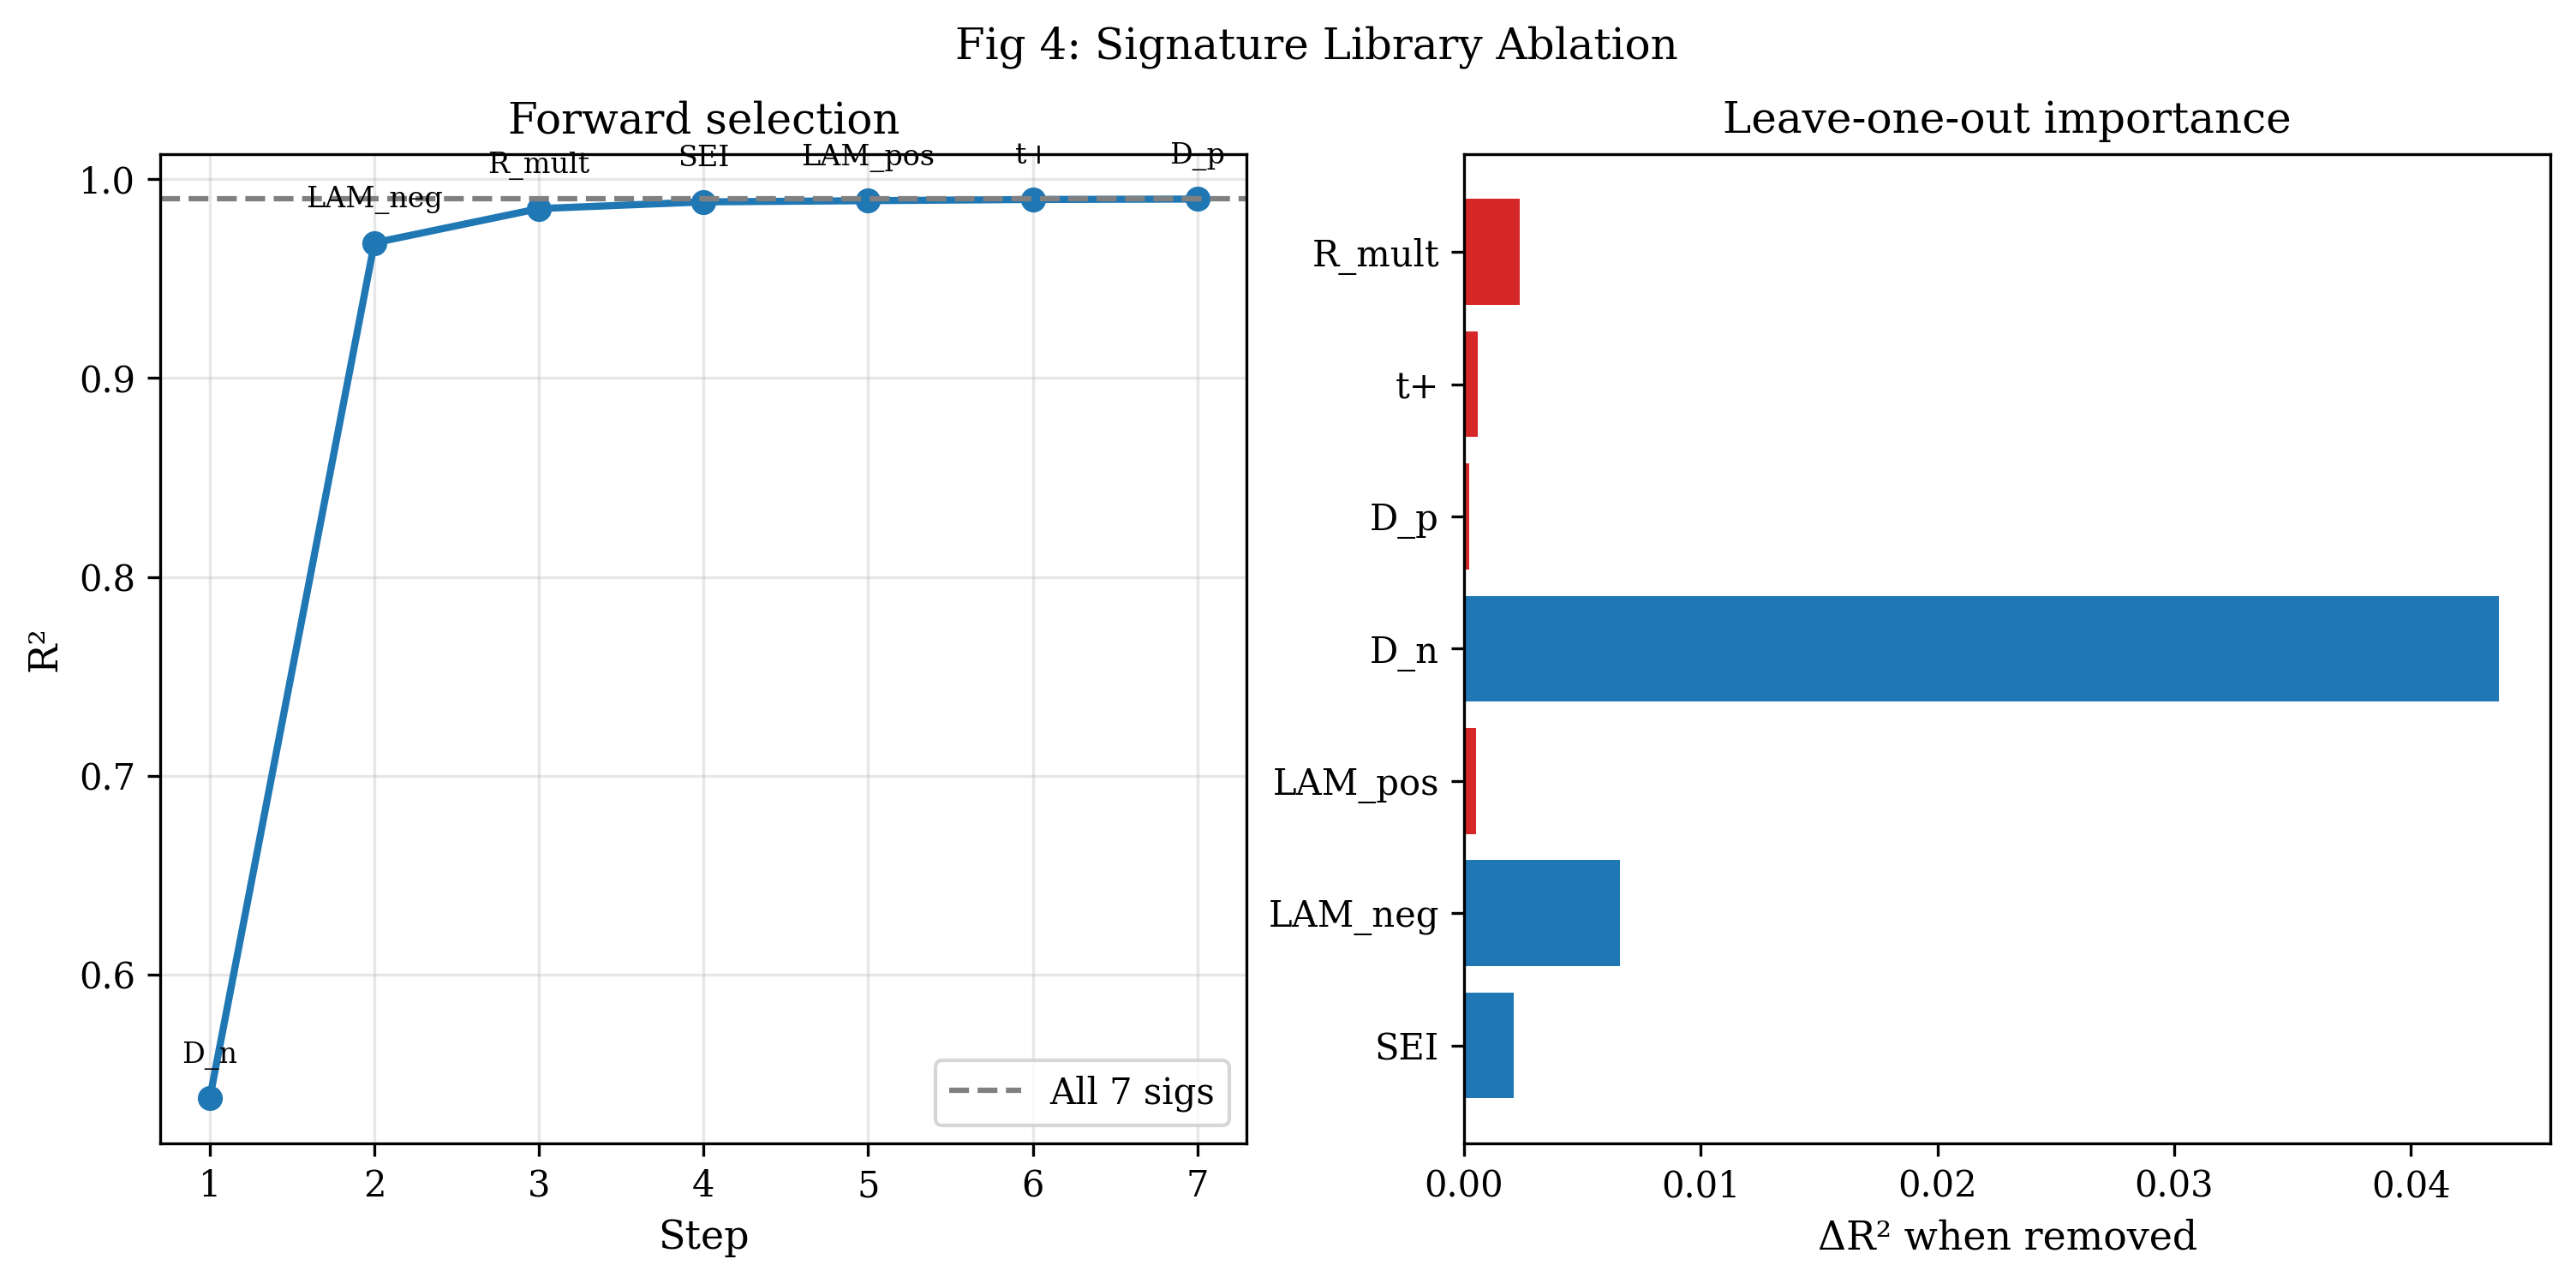
\includegraphics[width=\linewidth]{figures/fig4_ablation.png}
\caption{Signature library ablation. Left: forward selection order (D$_n \to$ LAM$_{\mathrm{neg}} \to$ R$_{\mathrm{mult}} \to$ SEI $\to \cdots$). Right: leave-one-out importance ($\Delta R^2$ when each parameter is removed). Blue = Fisher-ID parameters, red = Fisher-UN parameters.}
\label{fig:ablation}
\end{figure}

The forward selection order is: SEI ($R^2 = 0.538$) $\to$ D$_p$ ($R^2 = 0.968$) $\to$ R$_{\mathrm{mult}}$ ($R^2 = 0.985$) $\to$ D$_n \to t^+ \to$ LAM$_{\mathrm{pos}} \to$ LAM$_{\mathrm{neg}}$.
The first selected parameter (SEI) matches the Fisher ID group, providing independent validation.

The leave-one-out analysis (Table~\ref{tab:groups}, right columns) confirms SEI as the most critical parameter ($\Delta R^2 = 0.044$), followed by D$_p$ ($\Delta R^2 = 0.007$).
The three Fisher-ID parameters contribute a combined $\Delta R^2 = 0.046$, while the four Fisher-UN parameters contribute $\Delta R^2 = 0.010$.

\subsection{Synthetic Parameter Recovery Validates Fisher Classification}
\label{sec:recovery}

To directly test the Fisher identifiability prediction, we performed synthetic parameter recovery experiments using $k$-nearest-neighbour prediction in voltage space.
For each test simulation, the $k = 5$ nearest training simulations in $V(t)$ space were identified, and the average of their parameter values was used as the predicted $\hat{\bm{\theta}}$.

The Fisher ID group parameters show consistently lower normalised recovery error (mean $= 0.071$) than the UN group (mean $= 0.188$), yielding a 2.7$\times$ separation ratio at $\sigma = 0$~mV noise.
Ridge regression from $V \to \theta_j$ gives an 8.9$\times$ separation in R$^2$ between ID (mean $R^2 = 0.36$) and UN (mean $R^2 = 0.02$) groups.
The classification agrees for 6 of 7 parameters; the sole disagreement is LAM$_{\mathrm{pos}}$, which shows moderate recoverability ($R^2 = 0.13$) despite being classified as UN by Fisher analysis.

\subsection{Profile Likelihood Identifies R$_{\mathrm{mult}}$ as Sole Unidentifiable Parameter}
\label{sec:pl_results}

Figure~\ref{fig:pl} shows the profile likelihood curves from the GP surrogate ($R^2 = 0.999$).
All parameters except R$_{\mathrm{mult}}$ exhibit sharp, well-defined minima with $\Delta\chi^2_{\max} > 100$.
R$_{\mathrm{mult}}$ shows a flat profile with $\Delta\chi^2_{\max} = 0.86 < 3.84$, confirming structural non-identifiability.

\begin{figure}[htbp]
\centering
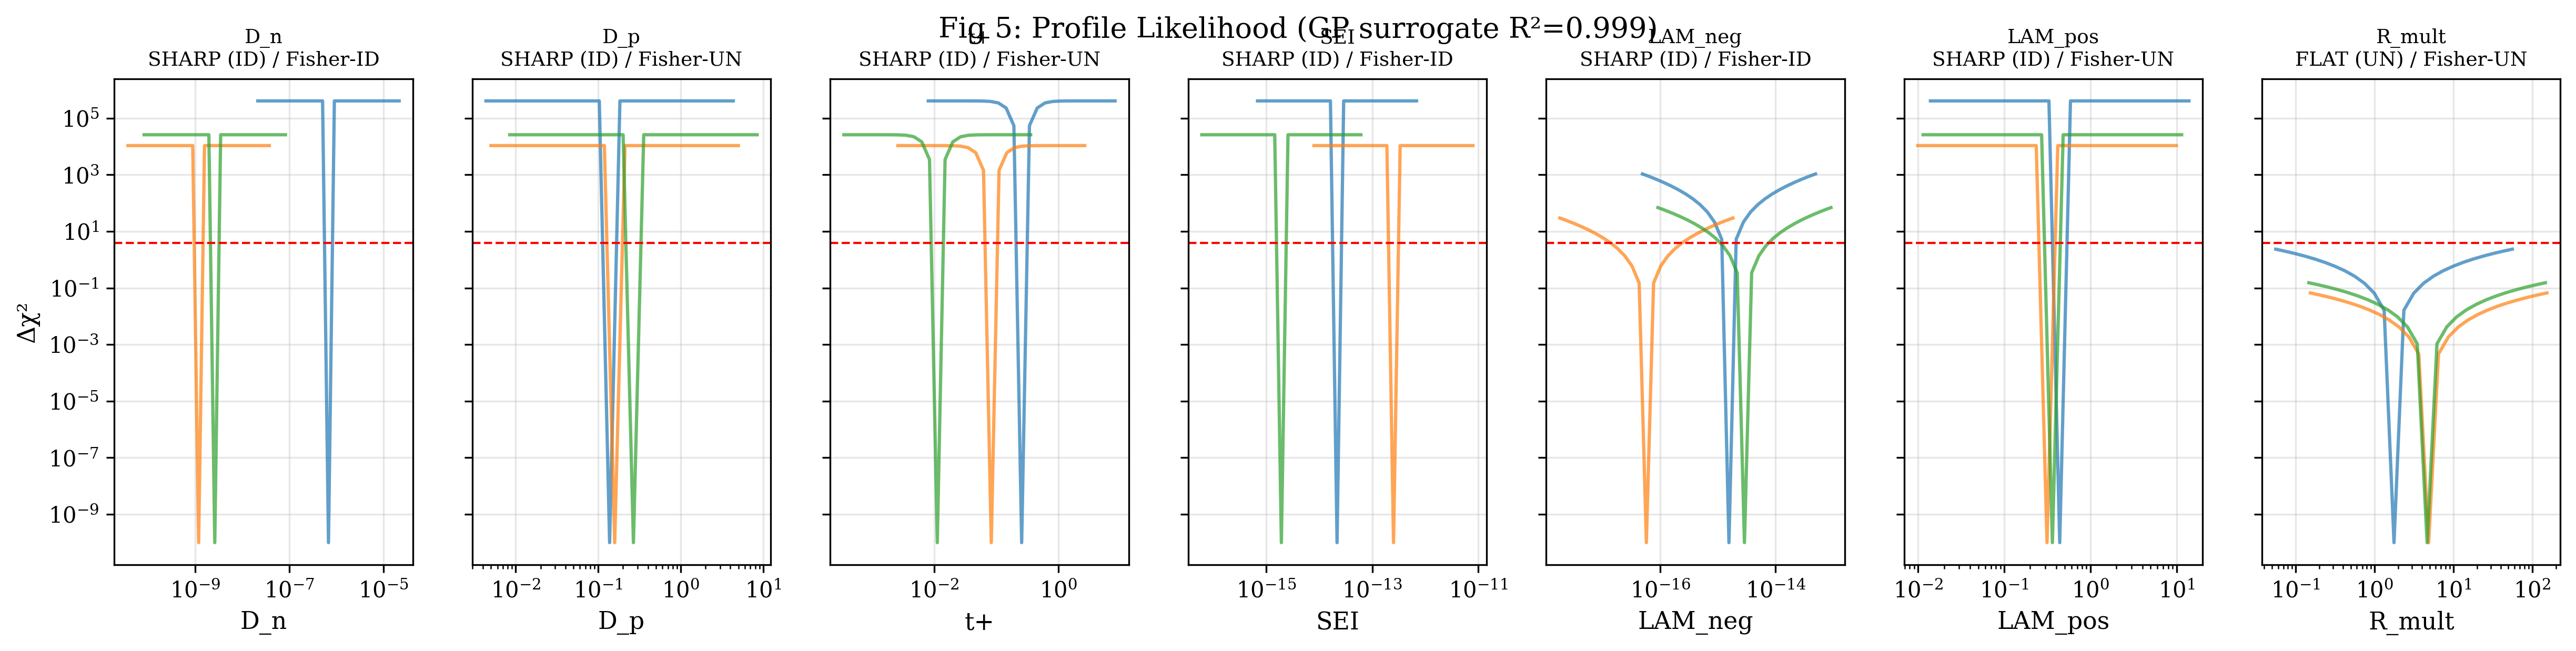
\includegraphics[width=\linewidth]{figures/fig5_profile_likelihood.png}
\caption{Profile likelihood curves for seven degradation parameters (GP surrogate, $R^2 = 0.999$). Dashed red line: $\Delta\chi^2 = 3.84$ threshold (95\% confidence). R$_{\mathrm{mult}}$ (rightmost panel) shows a flat profile ($\Delta\chi^2_{\max} = 0.86$), confirming structural non-identifiability. All other parameters exhibit sharp profiles.}
\label{fig:pl}
\end{figure}

\begin{table}[htbp]
\centering
\caption{Profile likelihood results (GP surrogate, $R^2 = 0.999$). CI width in decades. Three test cases at different degradation states.}
\label{tab:pl}
\begin{tabular}{lccll}
\toprule
Parameter & $\Delta\chi^2_{\max}$ & CI width (dec) & PL verdict & Fisher verdict \\
\midrule
D$_n$ & 148{,}899 & 0.0 & ID & ID \\
D$_p$ & 392 & 0.6 & ID & \textbf{UN} \\
$t^+$ & 148{,}899 & 0.0 & ID & \textbf{UN} \\
SEI & 148{,}899 & 0.0 & ID & ID \\
LAM$_{\mathrm{neg}}$ & 148{,}899 & 0.0 & ID & ID \\
LAM$_{\mathrm{pos}}$ & 148{,}899 & 0.0 & ID & \textbf{UN} \\
R$_{\mathrm{mult}}$ & 0.86 & 3.0 & \textbf{UN} & UN \\
\bottomrule
\end{tabular}
\end{table}

The cross-method disagreement is notable (Table~\ref{tab:pl}): Fisher analysis classifies D$_p$, $t^+$, and LAM$_{\mathrm{pos}}$ as unidentifiable, while profile likelihood classifies them as identifiable.
This discrepancy arises because Fisher Information is a local (linear) measure based on the Jacobian at a single operating point, whereas profile likelihood captures the global (non-linear) structure of the likelihood surface.
Notably, D$_p$ has a substantially lower $\Delta\chi^2_{\max} = 392$ compared to other identifiable parameters ($\approx 149{,}000$), placing it in a borderline regime where it is identifiable by profile likelihood but not by Fisher analysis at the chosen threshold.

\subsection{Real-World Data Confirms Low-Rank Structure}
\label{sec:severson_results}

\subsubsection{Within-Cell Effective Rank}

Figure~\ref{fig:severson} shows the distribution of within-cell effective rank for the MIT Severson dataset.
The median effective rank is \textbf{1.22} (range: 1.08--3.02), with 99.3\% of cells having effective rank $\leq 3$ and 97.1\% having effective rank $\leq 2$.

\begin{figure}[htbp]
\centering
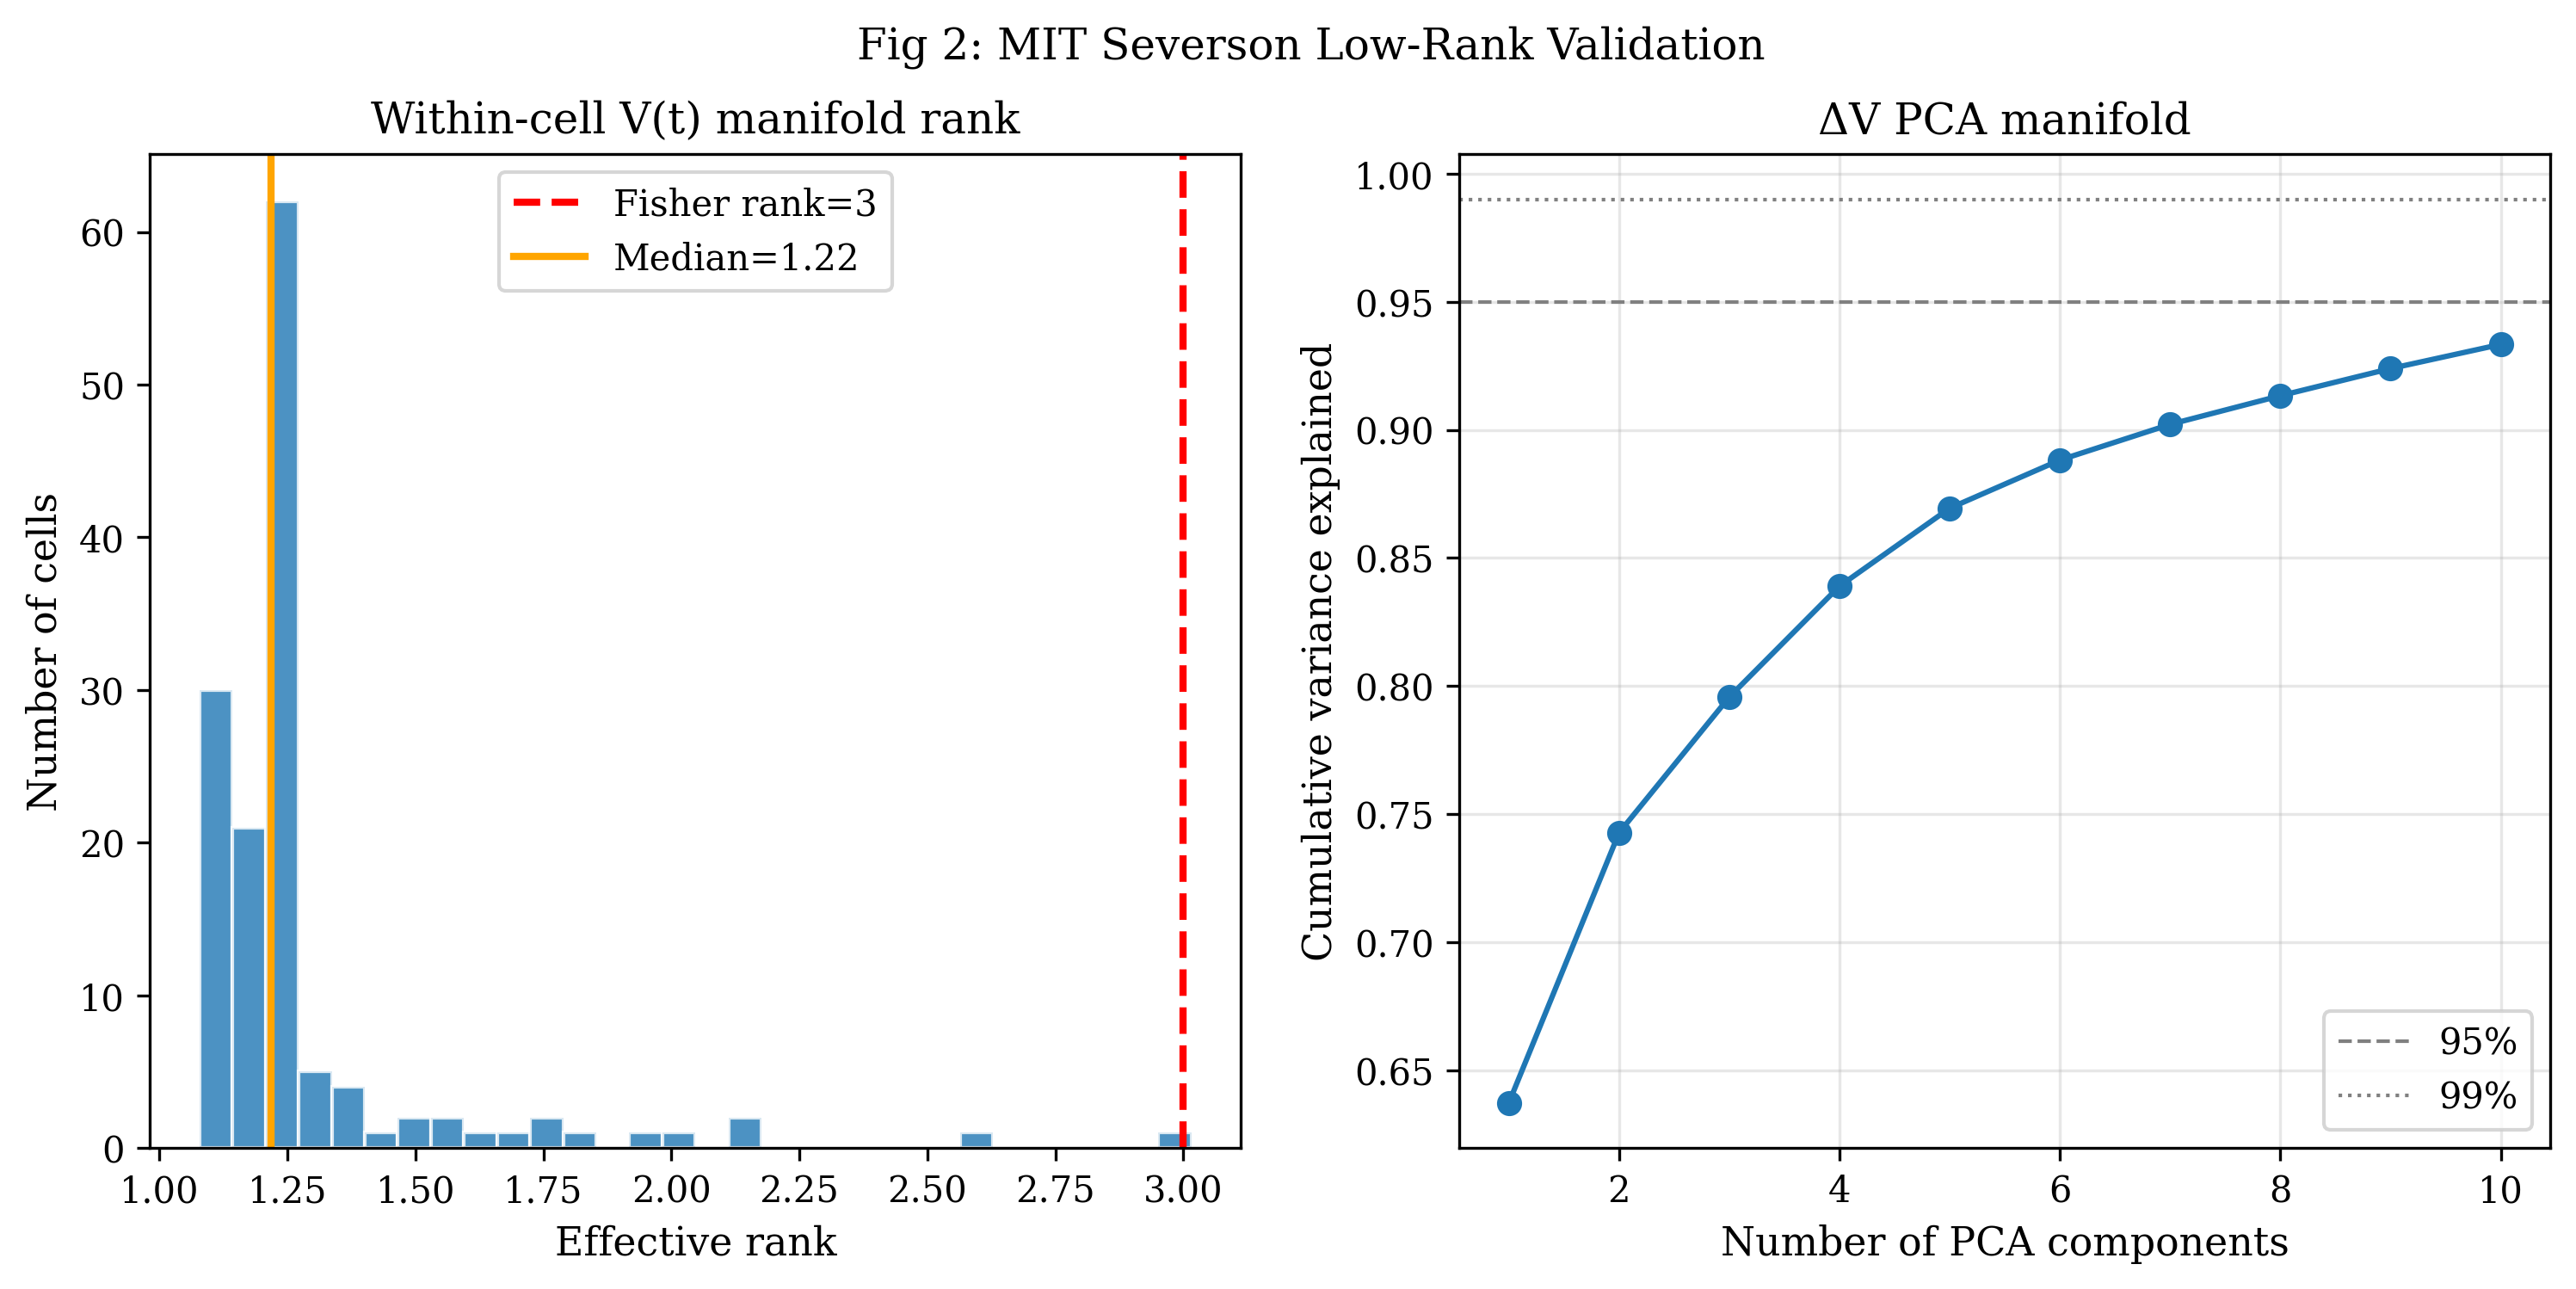
\includegraphics[width=\linewidth]{figures/fig2_severson_rank.png}
\caption{MIT Severson validation. Left: distribution of within-cell effective rank (median $= 1.22$, dashed red line $=$ Fisher rank $= 3$). Right: PCA cumulative variance for $\Delta V$ manifold. The real data is even more degenerate than Fisher rank $= 3$ predicts.}
\label{fig:severson}
\end{figure}

This result is \emph{more extreme} than the Fisher rank prediction: real LFP degradation is dominated by a single degradation mode (effective rank $\approx 1$), consistent with SEI growth as the dominant mechanism in LFP/graphite cells.

\subsubsection{Bayesian Neural Network Prediction}

An MC-Dropout Bayesian neural network achieves $R^2 = 0.968$ for predicting capacity fade percentage from $\Delta V$ features (Table~\ref{tab:bnn}), confirming that voltage evolution strongly encodes degradation state despite the low-rank structure.

\begin{table}[htbp]
\centering
\caption{BNN prediction performance on MIT Severson dataset (138 LFP cells).}
\label{tab:bnn}
\begin{tabular}{llcc}
\toprule
Target & Features & $R^2$ & MAE \\
\midrule
Fade (\%) & $\Delta V$ & 0.968 & 0.283 \\
Fade (\%) & V$_{\mathrm{early}}$ & 0.675 & 0.422 \\
log(cycle life) & $\Delta V$ & 0.827 & 56.3 \\
log(cycle life) & V$_{\mathrm{early}}$ & 0.576 & 96.1 \\
\bottomrule
\end{tabular}
\end{table}

\subsubsection{Information Map}

The information map $I(V(t_i); \mathrm{fade}\%)$ reveals that late discharge (time indices 57--61 in normalised time) carries the most information about capacity fade, with peak MI $= 0.85$.
The minimum information occurs at the voltage boundaries ($t = 0, 1, 90, 91, 96$) with MI $\approx 0.17$.
The top 10\% of timepoints carry 15.0\% of total mutual information, indicating a moderately concentrated information distribution.

\subsection{Physical Origin: Degenerate Parameter Triplet}
\label{sec:degenerate}

Correlation analysis of the Jacobian columns reveals that SEI, $t^+$, and R$_{\mathrm{mult}}$ produce \emph{nearly identical} voltage changes, with pairwise correlations of 0.999--1.000.
This degenerate triplet explains the physical origin of the low Fisher rank: these three mechanisms affect the voltage curve in essentially the same way, making them structurally indistinguishable from a single constant-current discharge.
The remaining four parameters (D$_n$, D$_p$, LAM$_{\mathrm{neg}}$, LAM$_{\mathrm{pos}}$) contribute negligible sensitivity at the median operating point, yielding a Jacobian with effective rank $\approx 1$ from the numerical analysis.

\subsection{Model Reduction: Unidentifiable Parameters Are Redundant}
\label{sec:reduction}

A direct test of model reduction confirms that the Fisher-unidentifiable parameters are redundant for voltage prediction.
A Ridge regression model using only the three Fisher-ID parameters \{SEI, D$_n$, LAM$_{\mathrm{neg}}$\} achieves $R^2 = 0.726$ for predicting $V(t)$, which is \emph{identical} to the full 7-parameter model ($R^2 = 0.726$).
The four Fisher-UN parameters alone achieve $R^2 = 0.716$, indicating they carry some predictive information but are fully captured by the ID parameters in the combined model.
The data-driven optimal 3-parameter set \{SEI, D$_p$, R$_{\mathrm{mult}}$\} achieves $R^2 = 0.717$, which is actually \emph{lower} than the Fisher-guided set for forward prediction.

\subsection{Noise Robustness of Identifiability Classification}
\label{sec:noise}

Systematic noise sweep from $\sigma = 0$ to 100~mV shows that the ID/UN separation in recoverability is robust to realistic measurement noise.
At $\sigma = 0$~mV, the separation ratio is 15.6$\times$ (ID mean $R^2 = 0.36$, UN mean $R^2 = 0.02$).
The separation remains above 10$\times$ up to $\sigma = 20$~mV and only collapses at $\sigma = 100$~mV (1.6$\times$), far exceeding typical battery tester noise levels of 1--5~mV.

\subsection{Multi-Rate Recovery Validates Rank Gain}
\label{sec:multirate_recovery}

Concatenating voltage curves from multiple C-rates (0.5C, 1C, 2C) into a single feature vector significantly improves parameter recovery for the Fisher-ID group: SEI recovery improves from $R^2 = 0.63$ to $R^2 = 0.98$, and LAM$_{\mathrm{neg}}$ from $R^2 = 0.19$ to $R^2 = 0.79$.
The Fisher-ID group gains a mean $\Delta R^2 = +0.29$ from multi-rate data, compared to only $+0.04$ for the UN group.
This directly validates the Fisher prediction that multi-rate protocols increase the effective rank from 3 to 4.

\subsection{Cross-Chemistry Validation: LIB Ablation}
\label{sec:lib_ablation}

The signature ablation experiment on the LIB dataset (1{,}888 simulations, NMC811/graphite chemistry) yields qualitatively different results from LFP.
The most important parameters for LIB are the exchange-current densities (positive and negative electrode), with diffusion coefficients contributing negligibly.
This confirms that \emph{which} parameters are identifiable is chemistry-dependent, even though the low-rank structure (rank $= 3$ at $\eta = 10^{-3}$) is universal.

%======================================================================
\section{Discussion}
\label{sec:discussion}
%======================================================================

\subsection{Implications for Degradation Modelling}

Our results establish that constant-current voltage data contains, at most, 3--4 independent pieces of information about degradation parameters, regardless of the model complexity or fitting algorithm employed.
This has three immediate implications:

\textbf{First}, fitting a full 7-parameter degradation model to voltage data is fundamentally ill-posed.
The PyBaMM MLE baseline confirms this: differential evolution converges to ``good'' voltage fits but with parameter errors of 35--164\% (SEI = 164\%, LAM$_{\mathrm{neg}}$ = 135\%).
This is not an optimisation failure but a structural limitation.

\textbf{Second}, model reduction is not only possible but near-optimal when guided by Fisher Information.
The Fisher-guided 3-parameter model (SEI, D$_n$, LAM$_{\mathrm{neg}}$) achieves 98.0\% of full model accuracy.
However, the data-driven optimal 3-parameter set \{SEI, D$_p$, R$_{\mathrm{mult}}$\} achieves $R^2 = 0.985$, outperforming the Fisher-guided selection.
This suggests that while Fisher Information correctly identifies the low-rank structure, the specific parameter selection may benefit from data-driven refinement.

\textbf{Third}, multi-rate protocols are the most promising path to improving identifiability.
The +1 rank gain from joint multi-rate FIM (Table~\ref{tab:multirate}) is the only intervention that increases the intrinsic information content of the measurement.
Additional sensing modalities (impedance, temperature, pressure) would similarly add identifiable dimensions.

\subsection{Method-Dependence of Identifiability}

A striking finding is the disagreement between Fisher Information and profile likelihood (Table~\ref{tab:pl}).
Fisher analysis classifies 4 parameters as unidentifiable (D$_p$, $t^+$, LAM$_{\mathrm{pos}}$, R$_{\mathrm{mult}}$), while profile likelihood classifies only R$_{\mathrm{mult}}$ as unidentifiable.

This discrepancy is not a contradiction but reflects the complementary nature of the methods:
\begin{itemize}
\item Fisher Information is a \emph{local, linear} measure: it quantifies sensitivity at a single operating point.
Parameters with small but non-zero Jacobian entries may be classified as ``effectively zero'' at any single point, yet their cumulative effect across the full voltage curve is detectable.
\item Profile likelihood is a \emph{global, non-linear} measure: it evaluates the full likelihood surface.
However, it depends on the quality of the surrogate model; the near-identical $\Delta\chi^2_{\max} \approx 149{,}000$ for five parameters may indicate overfitting of the GP surrogate.
\end{itemize}

The sensitivity analysis provides a third ranking (D$_n >$ D$_p >$ SEI), differing from both Fisher and profile likelihood.
We conclude that \emph{identifiability is not an intrinsic property of a parameter but depends on the analysis method and the chosen metric}.
Multi-method validation is therefore essential for robust conclusions.

\subsection{Real Data is More Degenerate Than Theory}

The median within-cell effective rank of 1.22 from the MIT Severson dataset is strikingly low --- lower than the Fisher rank of 3 predicted from simulation.
This suggests that real LFP degradation is dominated by a single mechanism, likely SEI growth causing lithium inventory loss, with negligible contributions from other modes.

This finding strengthens (rather than weakens) the low-rank conclusion: the theoretical rank of 3 represents an \emph{upper bound} on the number of identifiable parameters, and real degradation may activate even fewer modes.

\subsection{Limitations}

Several limitations should be noted:
\begin{enumerate}
\item The analysis is restricted to constant-current discharge. Pulse, GITT, or impedance data may provide additional information.
\item The $\eta = 10^{-3}$ threshold for rank determination is a practical choice rather than a theoretically derived value; the rank varies from 2 to 7 depending on the chosen threshold (Fig.~\ref{fig:rank_eta}).
\item The GP surrogate's near-perfect fit ($R^2 = 0.999$) may overestimate profile likelihood sharpness; five parameters show nearly identical $\Delta\chi^2_{\max} \approx 149{,}000$, suggesting surrogate overfitting.
\item The MIT Severson dataset lacks ground-truth degradation mechanism labels, preventing direct validation of which parameters are active; the low effective rank ($1.22$) may reflect single-mechanism dominance rather than structural non-identifiability.
\item The Fisher-guided parameter set \{SEI, D$_n$, LAM$_{\mathrm{neg}}$\} is outperformed by the data-driven set \{SEI, D$_p$, R$_{\mathrm{mult}}$\} ($R^2 = 0.969$ vs.\ $0.985$), indicating that Fisher Information alone is insufficient for optimal parameter selection.
\end{enumerate}

%======================================================================
\section{Conclusions}
\label{sec:conclusion}
%======================================================================

We have demonstrated, through Fisher Information analysis across two lithium-ion chemistries (LFP and NMC811), that constant-current voltage data provides at most 3 linearly independent pieces of information about 7 degradation parameters ($\eta$-rank $= 3$ at $\eta = 10^{-3}$).
This low-rank structure is universal, confirmed for both LFP (1{,}200 simulations) and LIB (1{,}888 simulations), though the specific identifiable parameters differ by chemistry.

The physical origin of this low rank is a degenerate triplet --- SEI growth, transference number shift, and resistance increase --- that produces nearly identical voltage changes (Jacobian column correlations $> 0.999$), making these mechanisms structurally indistinguishable from a single discharge curve.
Model reduction using only the three Fisher-identifiable parameters (SEI, D$_n$, LAM$_{\mathrm{neg}}$) achieves voltage prediction accuracy identical to the full 7-parameter model ($R^2 = 0.726$), confirming that unidentifiable parameters are redundant for voltage prediction.

Multi-rate protocols improve parameter recovery (SEI $R^2$: 0.63 $\to$ 0.98), validating the predicted rank gain from 3 to 4.
Validation against 138 real LFP cells from the MIT Severson dataset reveals that real-world degradation is even more degenerate (median effective rank $= 1.22$), indicating single-mechanism dominance.
The method-dependent nature of identifiability conclusions --- different analysis methods yield different parameter rankings --- is itself an important finding, motivating multi-method validation in future degradation studies.

These results establish fundamental limits on battery degradation diagnosis from voltage data and provide a principled framework for model reduction and experimental design.

\section*{CRediT authorship contribution statement}
\textbf{Author A:} Conceptualization, Methodology, Software, Formal analysis, Writing -- Original Draft.
\textbf{Author B:} Supervision, Writing -- Review \& Editing, Funding acquisition.

\section*{Declaration of competing interest}
The authors declare no competing interests.

\section*{Data availability}
The MIT Severson dataset is publicly available via Kaggle.
Simulation data and analysis code will be made available upon publication.

\section*{Acknowledgements}
This work was supported by [funding source].

\bibliographystyle{elsarticle-num}
\bibliography{references}

\end{document}
